\documentclass[10pt,twocolumn,letterpaper]{article}

\usepackage{cvpr}
\usepackage{times}
\usepackage{epsfig}
\usepackage{graphicx}
\usepackage{amsmath}
\usepackage{amssymb}
\usepackage{subfigure}

\newcommand{\myfrac}[2]{\textstyle\frac{#1}{#2}\displaystyle}

\long\def\symbolfootnote[#1]#2{\begingroup%
\def\thefootnote{\fnsymbol{footnote}}\footnote[#1]{#2}\endgroup} 

\newcommand{\TODO}{\textcolor{red}{TO DO:~}}
\newcommand{\KEVIN}{\textcolor{blue}{Kevin comment:~}}
\newcommand{\ALEX}{\textcolor{blue}{Alex comment:~}}
\newcommand{\JOHN}{\textcolor{blue}{Alex comment:~}}

\newcommand{\demi}{\myfrac{1}{2}}


\newcommand{\mysec}[1]{Section~\ref{sec:#1}}
\newcommand{\eq}[1]{Eq.~(\ref{eq:#1})}
\newcommand{\myfig}[1]{Figure~\ref{fig:#1}}
\newcommand{\myeq}[1]{Eq.~(\ref{eq:#1})}

\newcommand{\tr}{\text{tr}}
\newcommand{\vect}[1]{\text{vect}\left(#1\right)}

\newcommand{\diag}{\text{diag}}
\newcommand{\Diag}{\text{Diag}}

\newcommand{\xx}{\times}

\newcommand{\BEQAS}{\begin{eqnarray*}}
\newcommand{\EEQAS}{\end{eqnarray*}}

\newcommand{\BIEQAS}{\begin{IEEEeqnarray*}}
\newcommand{\EIEQAS}{\end{IEEEeqnarray*}}

\newcommand{\BEQA}{\begin{eqnarray}}
\newcommand{\EEQA}{\end{eqnarray}}

\newcommand{\BIEQA}{\begin{IEEEeqnarray}}
\newcommand{\EIEQA}{\end{IEEEeqnarray}}

\newcommand{\idm}{I}

\newcommand{\Simp}{\mathcal {S}}
\def\R{{\rm I}\!{\rm  R}}
\newcommand{\C}{\mathcal {C}}
\newcommand{\LL}{\ell}
\newcommand{\EE}{\mathbb {E}}
\newcommand{\Ecal}{\mathcal {E}}
\newcommand{\I}{\mathbbm {1} }

\newcommand{\mcal}[1]{\mathcal{#1}}
\newcommand{\bb}[1]{\mathbb{#1}}

\newcommand{\Fa}{J_{\alpha}}
\newcommand{\Fwb}{J_{w b}}
\newcommand{\Fapp}{J_{\text{app}}}


\newcommand{\suce}{\preccurlyeq}
\newcommand{\estSuce}{\succcurlyeq}

\newcommand{\logPartNS}{A_0(W,b)}
\newcommand{\logPart}[1]{A_{#1}(W,b)}
\newcommand{\psiPara}{\tau}

\newcommand{\sumL}{\sum_{l=1}^K}
\newcommand{\sumK}{\sum_{k=1}^K}
\newcommand{\sumN}{\sum_{n=1}^N}
\newcommand{\sumM}{\sum_{m=1}^M}
\newcommand{\sumR}{\sum_{r=1}^R}
\newcommand{\sumP}{\sum_{p=1}^P}
\newcommand{\sumKL}{\sum_{k,k'=1}^K}

\newtheorem{theorem}{Theorem}[section]
\newtheorem{proposition}[theorem]{Proposition}

\newcommand{\BITE}{\begin{equation}\left\{ \begin{array}{lll}}
\newcommand{\EITE}{\end{array}\right.\end{equation}}

\newcommand{\BITES}{\begin{equation*}\left\{ \begin{array}{lll}}
\newcommand{\EITES}{\end{array}\right.\end{equation*}}






% Include other packages here, before hyperref.

% If you comment hyperref and then uncomment it, you should delete
% egpaper.aux before re-running latex.  (Or just hit 'q' on the first latex
% run, let it finish, and you should be clear).
\usepackage[pagebackref=true,breaklinks=true,letterpaper=true,colorlinks,bookmarks=false]{hyperref}

% \cvprfinalcopy % *** Uncomment this line for the final submission

\def\cvprPaperID{304} % *** Enter the CVPR Paper ID here
\def\httilde{\mbox{\tt\raisebox{-.5ex}{\symbol{126}}}}

% Pages are numbered in submission mode, and unnumbered in camera-ready
\ifcvprfinal\pagestyle{empty}\fi
\begin{document}

%%%%%%%%% TITLE
\title{Attend to the player: Player attention for event detection}

\author{First Author\\
Institution1\\
Institution1 address\\
{\tt\small firstauthor@i1.org}
% For a paper whose authors are all at the same institution,
% omit the following lines up until the closing ``}''.
% Additional authors and addresses can be added with ``\and'',
% just like the second author.
% To save space, use either the email address or home page, not both
\and
Second Author\\
Institution2\\
First line of institution2 address\\
{\tt\small secondauthor@i2.org}
}

\maketitle
%\thispagestyle{empty}

%%%%%%%%% ABSTRACT
\begin{abstract}
Multi-player event recognition is a challenging task, particularly in sports
where many players are active in the scene but only a small subset
contribute to the event. In this paper, we propose a model which learns to
detect events in basketball videos while automatically "attending" to the
players responsible for the events. We detect players in videos and learn
time-varying attention weights to combine their features at each time-instant.
The attended features are then classified with a Long Short-Term Memory (LSTM)
model.  We explore two variants of attention models based on the need for
player-tracking.  We also propose a new basketball dataset comprised of 257
basketball games with 14K event annotations corresponding to 11
event classes.  Our model outperforms state-of-the-art methods for both event
classification and detection on this new dataset. Additionally, we also present
quantitative and qualitative evaluation of our model's attention performance.
Through these experiments we demonstrate the interpretability and utility of
the attention scores generated by our model.
\end{abstract}

%%%%%%%%% BODY TEXT
\section{Introduction}
When observing a scene, we posess the inate ability to filter out unwanted
stimuli \cite{Desimone_ARN95} and focus only on a selected subset of objects.
This effect is easily understood in the context of multi-player sports, where
we look at only a few key players (Fig.~\ref{fig:pull_figure}) to understand a
complete event. Motivated by this observation, we present an event detection
method which automatically ``attends" to the most releavant person during
different phases of a multi-player event.

\begin{figure}[ht!]
\begin{center}
\fbox{\rule{0pt}{2in} \rule{.9\linewidth}{0pt}}
\end{center}
   \caption{Pull figure.}
\label{fig:pull_figure}
\end{figure}

Acitivity and event recognition in videos has hugely benefited with the
introduction of many recent large scale datasets \cite{}. However, most of
these dataset focus on activities performed by a single person.  Multi-person
datasets like \cite{} are usually restricted to fewer videos.  Further, to
evaluate event detection, it is desirable to have temporal annotations in long
untrimmed videos. Since the focus of our work is towards multi-person actions,
we propose a new dataset of basketball events with time-stamp annotations for
all occurrences of $11$ different events across $257$ videos each $1.5$ hours
long in length.  This dataset is comparable to the THUMOS \cite{THUMOS}
detection dataset in terms of number of annotations and contains longer videos
catering to a multi-person setting.

In basketball, many players are always present in the court.
However, an interesting event like a ``layup" or ``steal" can be attributed
to just one or two players at the scene. Observing these people at the right
time holds the cue to understanding the entire event. Furhter, identifying
these players responsible for the event is an interesting task in its own right.
Hence, it is natural to develop a model which can ``attend" to these players during
an event.

Recently, Recurrent Neural Network (RNN) models have been successful in
using ``attention" \cite{Bahdnau_arxiv14,Xu_arxiv15,Yao_arxiv15} for aligning
elements from an input sequence to those of an output sequence. In these settings,
the input sequence remains fixed at all times and the model chooses from this
fixed input at each instant. However, the use of such attention based RNNs
poses two challenges in our setting:
1. The set of player detections varies from one frame to the other and
2. The model needs to adapt attention according to the phase of the game as
shown in Fig.~\ref{fig:pull_figure}. This presents interesting choices
for the attention model.

While it is possible to treat player detections across frame to be
disconnected, in practice the detections belong to the same set of plyers. We
could leverage this knowledge by using a player tracker followed by better
player representations. However, this could lead to additional issues due to
erroneous tracking and could possibly lower the effectiveness of attention
itself. On the other hand, it is more lucrative to develop an attention model
without tracking.  This could provide more freedom to switch attention between
detections based on the state of the event. We explore both these choices in
our work and compare their event recognition performance as well as ability to
attend to the right players.

The main contribution of our works is to:
1. present a time-varying attention model for basketball event detection
in the presence and absence of player-tracking, 2. We provide a comprehensive
evaluation of the attention scores generated by our model and show
their interpretability in our setting and 3. We introduce a novel
large-scale basketball event dataset with 14K dense temporal annotations
for long video sequences. We outpuerform state-of-the-art
event recognition methods on the new dataset.


\section{Related Work}

\noindent \textbf{Action recognition in videos}
Traditionally, well engineered features have proved quite effective for video
classification and retrieval tasks
\cite{Dalal_ECCV06,Jain_CVPR13,Jiang_ECCV12,Laptev_CVPR08,
Niebels_ECCV10,Oh_MVA14,Oneata_ICCV13,Peng_ECCV14,Sadanand_CVPR12,Wang_BMVC09,Wang_CVPR11}.
The improved dense trajectory (IDT) features \cite{Wang_CVPR11} achieve
competetive results on standard video datasets.  In the last few years,
end-to-end trained deep netowork models
\cite{Ji_PAMI13,Karpathy_CVPR14,Simonyan_2014,Tran_arxiv14} were shown to be comparable and
at times better than these features for various video tasks.  Other works like
\cite{Xu_2015,Zha_2015,Wang_arxiv15} explore methods for pooling such
features for better performance.

Recent works using Recurrent Neural Networks (RNN) have achieved
state-of-the-art results for both event recognition and caption-generation
tasks \cite{Donahue_arxiv14,Ng_arxiv15,Srivastava_2015,Yao_arxiv15}.
We follow this line of work with addition of attention mechanism
to attend to the event particiapants.

\noindent \textbf{Attention models}
Itti et al. \cite{Itti_PAMI98} explored the idea of saliency based attention in
images, with other works like \cite{Shapovalova_NIPS13} using eye-gaze data as
a means for learning attention.
Other approaches such as Gkioxari et al. \cite{Gkioxari_arxiv14} and Raptis et al. \cite{Raptis_CVPR12}
automatically localize a spatio-temporal tube in the video corresponding to the action.

Recently, \cite{Bahdnau_arxiv14} showed that
attention based RNN models can effectively align input words in a sentence to
output words for machine translation.  Following this work, attention was used
for aligning regions in an image to output words for image-cpationing
\cite{Xu_arxiv15} and frames in a video with output words for video-captioning
\cite{Yao_arxiv15}.  In all these methods, attention aligns a sequence of input
features with words of an output sentence. However, in our work we use
attention to identify the most releavant person to the overall event during
different phases of the event.  Further, in our setting the attended set of
player detections changes between frames. This leads to interesting model choices.

\noindent \textbf{Action recognition datasets}
Action recognition in videos has eveolved with the introduction of more
sophisticated datasets starting from smaller KTH \cite{KTH}, HMDB \cite{HMDB}
to larger , UCF101 \cite{UCF101}, TRECVID-MED \cite{MED11} and Sports-1M \cite{Karpathy_CVPR14}
datasets.
More recently, THUMOS \cite{THUMOS} and ActivityNet \cite{ActivityNet} also provide a detection
setting with temporal annotations for actions in untrimmed videos.
There are also fine-grained datasets
in specific domains such as MPII cooking \cite{Finegrained_cooking} and breakfast \cite{Breakfast}.
However, most of these dataset focus on single-person activities with hardly
any need for recognizing the people responsible for the event. On the other
hand, publicly available multi-person activity datasets \cite{Choi_ICCV09,Ryoo_10} are restricted
to a very small number of videos.  One of the contributions of our work is 
a multi-player basketball dataset with dense temporal event annotations in
long videos. We provide more details in the next section.

\section{NCAA Basketball Dataset}
We are not only interested in detecting events in long untrimmed videos, but
also automatically identifying the people responsible for the events.

Unfortunately, recent activity detection datasets like THUMOS \cite{THUMOS},
ActivityNet \cite{ActivityNet}, and others such as
\cite{UCF101,Finegrained_cooking} mostly contain videos with a single actor
where every action is performed in a different setting. These are actions from
multiple sports events and/or household chores.  Identying the person
responsible for the action is not an interesing task in these datasets, and is
not critical for recognizing the action itself.

We focus on a multi-person setting where the events can be primarily
differentiated by the action of a small subset of people present in the scene.
Here, attending to the releavant people becomes more crucial and is a valuable
output in itself. A natural choice for such events is a multi-player sport.
With this in mind, we have collected a new large-scale dataset of basketball
events. This dataset will be made publicly available upon publication.

\subsection{Data Collection}
We needed a large collection of publicly available videos to construct the dataset.
Incidentally, complete basketball videos are
publicly available for $296$ NCAA games on
YouTube\footnote{https://www.youtube.com/user/ncaaondemand}.  These games are
played in different venues over different periods of time with a good amount of
diversity in setting and gameplay across the videos. More interestingly, they
are also accompanied by sparse play-by-play text snippets describing the events
at a few key-moments in each game.

We only consider the most recent $257$ games and ignore the older games with
slightly different rules than modern basketball.  As a first step, we clustered the
play-by-play text to identify the most frequent events from all games. We
narrowed the event list to $11$ classes. These included 5 types of shots and
steal, with each shot being further classified as a successful or failed
attempt (Fig.~\ref{fig:data_dist}). We then setup an AMT task, where the
annotators were asked to annotate the ``end-point" of these events if and when
they occur in the videos. Most basketball shots are of fixed duration. Hence,
we treat a 4 second window around the annotated ``end-point" as the total span
of the event.  Refer to supp. material for more details of the AMT task.

The videos were randomly split into $212$ training, $12$ validation and $33$
test videos. This accounted for a total of $11436$ training, $856$ validation
and $2256$ test event annotatoins. Note that the total number of training and
validation event annotations are comparable to the ongoing THUMOS'15 detection
challenge ($XXXX$ trimmed training instances for $20$ classes and $6553$
untrimmed validation instances). The distribution of annotations across all the
different events is visualized in Fig.~\ref{fig:data_dist}, with sample videos
for a few event classes. The annotations cover all occurrences of the
events in each video. The videos are typically $1.5$ hours long.  To the best of our
knowledge, this is the first dataset with dense temporal annotations for
such long video sequences.

\section{Our Method}

% -------- Heat Map for youtube videos
\begin{figure*}[t!]
\begin{center}

   \subfigure[Attention without tracks]{
                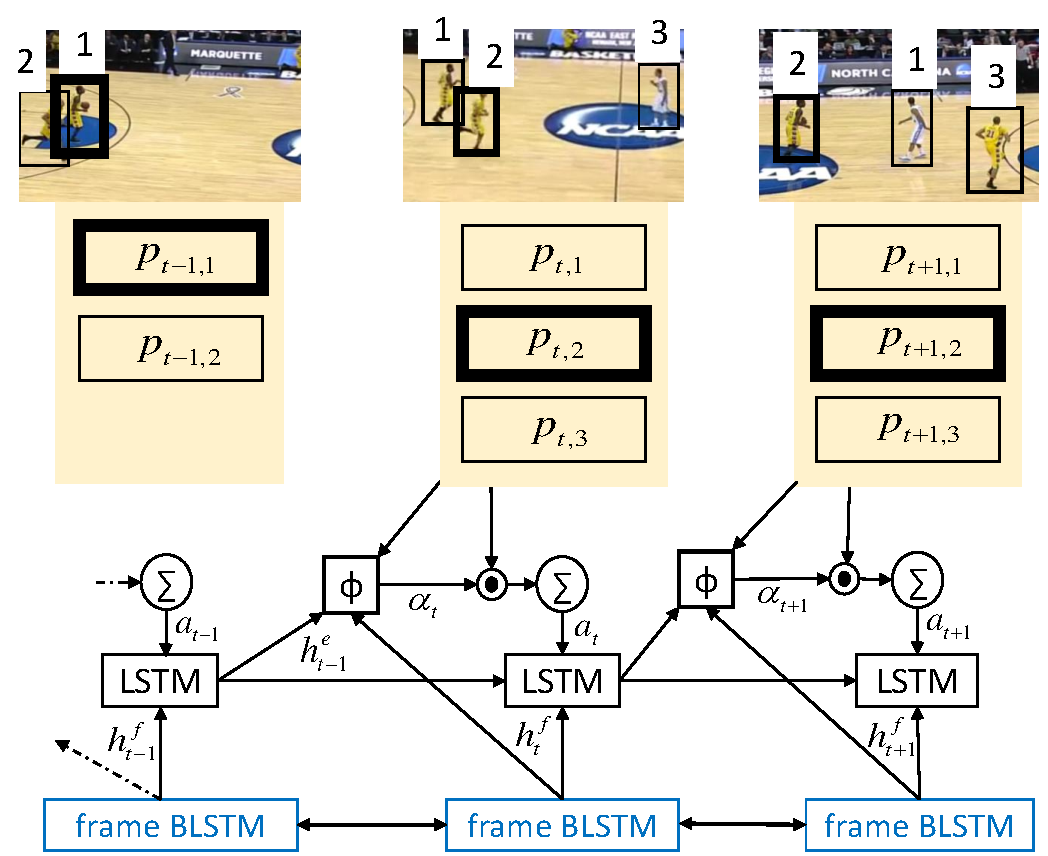
\includegraphics[width=3 in]{images/system_figure_2_cropped.pdf}
                \label{fig:heatmap_ft}
    }
   \subfigure[Attention with tracks]{
                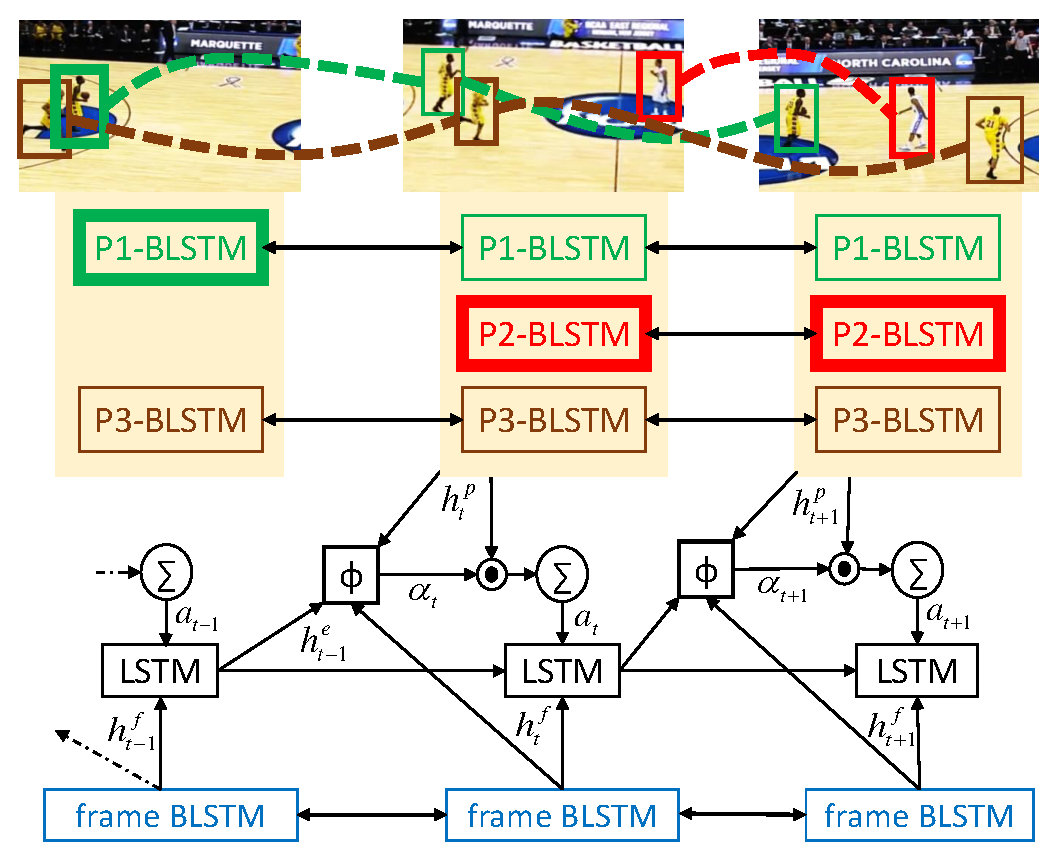
\includegraphics[width=3 in]{images/system_figure_1_cropped.pdf}
                \label{fig:heatmap_lp}
    }
\end{center}
   \caption{Our attention models (a) without tracks and (b) with tracks are
   shown here. The variables in the model are explained in the methods
 section.}
\label{fig:att_heatmap}
\end{figure*}
% ---------------------------------------------------------------------------------


All events in a basketball game are performed in the same scene by the same set
of players. The only basis for differentiating these events is the action
pefromed by a small subset of players at a given time.  For instance, a
``steal" event is completely defined by the action of the player attempting to
pass the ball and the player stealing from him.  To understand such an event,
it is sufficient to observe only these players pariticipating in the event.

This motivates us to build a model which can reason about an event by focusing
on specific players during the different phases of the game.  Such a foucsing
mechanism would also provide valuable information about the game-state, making
the model more interpretable.

\subsection{Player detection and feature extraction}
Given a set of basketball video clips, we first preprocess the clips to extract
player bounding boxes and features. We train a Multibox model \cite{} to detect
basketball players with bounding-box annotations collected on a subset of
training video frames. This model is then run on all frames of the training and
test videos to extract player bounding boxes.

A video clip $v$ is represented by a sequence of $D_f$ dimensional
frame-features $f_t$ extracted at each time-step $t$, as well as a set of $D_p$
dimensional player features $\mathcal{P}_t$ extracted from the player bounding
boxes at time $t$.

\begin{eqnarray}
  v & = & \left[ \left(f_1, \mathcal{P}_1\right), \dots,
\left(f_T, \mathcal{P}_T\right) \right]\;,\;\;f_t \in \mathbb{R}^{D_f} \\ \nonumber
\mathcal{P}_t & = & \{ p_{t1}, \dots, p_{t{P_t}} \}\;,\;\;p_{ti} \in \mathbb{R}^{D_p} \nonumber
\end{eqnarray}whre $P_t$ is the number of boxes at time $t$ and $T$ is the number of frames
in the video.

The frame feature $f_t$ is the activation of the last fully connected layer of
GoogLeNet \cite{} trained on ImageNet \cite{}.  The player feature $p_t^j$
contains both appearance and spatial components. The appearance features were
extracted by feeding the cropped and resized player region from the frame
through GoogLeNet and spatially pooling the response from a lower layer. The
spatial feature corresponds to a spatial histogram indicating the bounding box
location.  We explain this feature representation in more detail in the
supplementary material.

\subsection{LSTM event classifier}
Given a video $v$, we pass the frame-level features $f_t$ at time $t$ through a
Bidirectional Long Short-Term Memory (BLSTM) network. This helps in combining
contextual information from adjacent frames to provide a better frame
representation.  Let the hidden state of this BLSTM at time $t$ be denoted by
$h^f_t$.  This is the concatenated hidden state from both the forward and the
reverse LSTMS of the BLSTM. Refer to supp.  material for more details.

In order to attend to specific players in each frame, we pass the player features
through our attention model to generate an attention weighted player feature
$a_t$. The attention model is the main contribution of our work
and is explained in detail in the next section.

We feed the concatenated vector $[h^f_t, a_t]$ to a final event classification
LSTM, similar to the LRCN \cite{} model for video classification. Let
the hidden state of this LSTM at time $t$ be represented by $h^e_t$.  We then
train the model by minimizing the following one-vs-all hinge loss:

\begin{equation}
  L = \sum_{k = 1}^K \max (0, 1 - y_k w_k \cdot h^e_t)^2,
\end{equation} where $y_k$ is $1$ if the video belongs to class $k$,
else it is $-1$, and the weight vector corresponding to
class $k$ is denoted by $w_k$.

\subsection{Attention models}

Unlike past attention models \cite{}, we need to attend to a different set of
features at each time-step. There are two key issues to address in this
setting.

First, although we have different set of detections in each frame, the player
detections can be connected across the frames through an object tracking
method. This could potentially lead to better feature representation of the
players.

Second, player attention depends on the state of the event and needs to evolve
with the event.  For instance, during the start of a ``free-throw" it is
important to attend to the player making the shot. However, towards the end of
the event the success or failure of the shot can be judged by observing the
person in posession of the ball.

With these issues in mind, we explore two models:
one without an object tracker and the other using an object tracker.

\noindent \textbf{Player attention without tracking}
Here, we treat the detections in each frame to be independent from other
frames.  This alows the model to be more flexible in switching attention
between players as the event progresses.  As we later observe empirically, this
leads to better interpretability.  Also, the model does not suffer from
tracking errors.

At each time-step $t$, this model selects from the set of player features
$\mathcal{P}_t$. The attention is decided by a softmax weighting:

\begin{eqnarray} \label{eq:notrack}
  a_t & = & \sum_{i=1}^{P_t} \alpha_{ti} p_{ti} \\ \nonumber
  \alpha^{ti} & = & \text{softmax} \left(\phi\left(h^f_t, p_{ti}, h^e_{t-1}\right)\right),
\end{eqnarray}where the attention value $\alpha_{ti}$ for the $i^{th}$ player
detection at $t$ is decided by a softmax over the player scores $e_{ti}$. This
score is obtained from a multi layer perceptron $\phi$, similar to
\cite{Bahdnau_arxiv14}. Refer to the supp. material for details.

\noindent \textbf{Player attention with tracking}
In this model, we first associate the detections across all the frames to
obtain tracks corresponding to each player in the video.  We use a
standard multi-object tracker with bipartite matching to obtain the tracks
Fig.\ref{fig:track_specific_model}.

The player-track is a temporal sequence representing the change in position and
appearance of the player with time.  We could use this to gain a better
representation for the player which incorporates temporal context from all
frames. Hence, we pass the features corresponding to the bounding box of the
track at each time-step through a BLSTM as shown in
Fig.~\ref{fig:track_specific_model}. Let the hidden state of this ``player"
BLSTM corresponding to the $k^{th}$ track be denoted by $h^p_{tk}$. Similar to
Eq.~\ref{eq:notrack}, the attention-weighted $a_t$ feature is given by:

\begin{eqnarray}
  a_t & = & \sum_{i=1}^{P_t} \alpha_{ti} h^p_{ti} \\ \nonumber
  \alpha^{ti} & = & \text{softmax} \left(\phi\left(h^f_t, h^p_{ti}, h^e_{t-1}\right)\right),
\end{eqnarray}

While this provides a more consistent representation for the players across frames,
this model could suffer from wrong associations due to trakcing. This in turn makes
the interpretation of attention scores more difficult.

\section{Experiments}
In this section, we present three sets of experiments on the NCAA basketball
dataset: 1. event classification, 2. event detection and 3. evaluation of
attention. Note that previous attention models have typically shown selected
qualitative results to visualize attention in their settings. However, few
attempts have been made to quantitatively evaluate attention. A key
contribution of our paper is to provide both a qualitative and a quantitative
analyis of the attention scores.

\subsection{Implementation details}
We preprocess all videos to remove close up shots of players, animations as
well as crowd shots through a separate classifier. Refer to supp. material for
more details.  The hyperparameters were chosen by cross-validating on the
validation set.  We used a hidden state dimension of $256$ for all the LSTM and
BLSTM RNNs, an embedding layer with ReLU non-linearity and $256$ dimension for
embedding the player features and frame features before feeding to the RNNs.
All the event videos clips were four seconds long and subsampled to 6fps.  The
$\beta$ value was set to $0.5$ for the attention softmax weighting. We used a
batch size of $128$, learning rate of $0.005$ which was reduced by a factor of
$0.1$ every $10000$ iterations with RMSProp\cite{RMSProp}. The models were trained on
a cluster of $20$ GPUs for $100k$ iterations over one day.

\subsection{Event classification}
We train models for event classification with the annotated examples
from the basketball training set. In this setting, we do not use any
additional negatives from other parts of the basketball videos. This
is the typical classification setting, where we try to classify a
video into one of eleven classes. The mean average precision (mAP)
are shown in Tab.~\ref{tab:class_res}. We compare our results
against different control settings and baseline models as explained
below:


\begin{table*}[t!]
\begin{center}
\small
 \begin{tabular}{|l|c|c|c|c|c|c|c|c|c|}
  \hline
Event & IDT\cite{Wang_CVPR11} & IDT\cite{Wang_CVPR11} player & C3D \cite{Tran_arxiv14} & LRCN \cite{Donahue_arxiv14} & MIL\cite{} & Only player & Avg. player & Our no track & Our with track \\ \hline \hline

3-point succ.    & 0.501 &  & 0.282 & 0.462 &  & 0.469 & 0.545 & 0.583 & 0.600 \\
3-point fail.    & 0.370 &  & 0.117 & 0.564 &  & 0.614 & 0.702 & 0.668 & 0.738 \\
fr-throw succ. & 0.365 &  & 0.319 & 0.876 &  & 0.885 & 0.809 & 0.892 & 0.882 \\
fr-throw fail. & 0.778 &  & 0.642 & 0.584 &  & 0.700 & 0.641 & 0.671 & 0.516 \\
layup succ.      & 0.278 &  & 0.185 & 0.463 &  & 0.416 & 0.472 & 0.489 & 0.500 \\
layup fail.      & 0.283 &  & 0.195 & 0.386 &  & 0.305 & 0.388 & 0.426 & 0.445 \\
2-point succ.    & 0.303 &  & 0.254 & 0.257 &  & 0.228 & 0.255 & 0.281 & 0.341 \\
2-point fail.    & 0.136 &  & 0.078 & 0.378 &  & 0.391 & 0.473 & 0.442 & 0.471 \\
sl. dunk succ.  & 0.004 &  & 0.004 & 0.285 &  & 0.107 & 0.186 & 0.210 & 0.291 \\
sl. dunk fail.  & 0.197 &  & 0.047 & 0.027 &  & 0.006 & 0.010 & 0.006 & 0.004 \\
steal            & 0.555 &  & 0.303 & 0.876 &  & 0.854 & 0.894 & 0.886 & 0.893 \\ \hline \hline
Mean             & 0.343 &  & 0.221 & 0.469 &  & 0.452 & 0.489 & 0.505 & 0.516 \\ \hline
  \end{tabular}
\end{center}
  \caption{Mean average precision for event classification on the NCAA basketball dataset.}
  \label{tab:event_class}
\end{table*}

\begin{itemize}
  \item \emph{IDT\cite{Wang_CVPR11}} We use the publicly available implementation of dense trajectories with
  Fisher encoding.
  
  \item \emph{IDT\cite{Wang_CVPR11} player} We use IDT along with averaged features extracted from the player
  bounding boxes.

  \item \emph{C3D \cite{Tran_arxiv14}} We use the publicly available pre-trained model for feature extraction
  with a SVM classifier.

  \item \emph{LRCN \cite{Donahue_arxiv14}} This is a baseline model where we use a simple BLSTM on frame-level features similar
  to LRCN. The only difference is the use of BLSTM in place of LSTM. We found this to improve
  performance.

  \item \emph{MIL \cite{}} Since each frame can be seen as a bag of player features, we used the
  classical MIL model. Refer to supp. material for details.

  \item \emph{Only player} We only use player features without frame-level
  features in our model.
 
  \item \emph{Avg. player} In this control setting, we combine the player features by averaging without
  attentoin.

  \item \emph{Our no track} Our attention model without tracks.

  \item \emph{Our with track} Our attention model with tracking.
\end{itemize}



\subsection{Event detection}
In addition to classification, we also test our model for temporal detection performance
in the basketball dataset.
We use a sliding window approach, where we slide a $4$ second window
through all the $190$ basketball videos and try to classify the window into a negative
class or one of the 11 event classes. We use a stride length of $2$ seconds.
We treat all windows which do not overalp more than $1$ sec with any of the $11$ annotated
events as negatives. We use the same setting for training, test and validation.
This leads to $90200$ negative examples across all the videos. The detection results
are presented in Tab.~\ref{tab:detection_res}. We compare with the same baselines as before.

\begin{table*}[ht!]
\begin{center}
\small
 \begin{tabular}{|l|c|c|c|c|c|c|c|c|c|}
  \hline
Event & IDT\cite{Wang_CVPR11} & IDT player\cite{Wang_CVPR11} & C3D \cite{Tran_arxiv14} & LRCN \cite{Donahue_arxiv14} & MIL\cite{} & Only player & Avg. player & Our no track & Our with track \\ \hline \hline
3-point succ.  &  &  &  & 0.505 &  & 0.526 & 0.521 & 0.556 & 0.600 \\
3-point fail.  &  &  &  & 0.230 &  & 0.251 & 0.268 & 0.263 & 0.239 \\
fr-throw succ. &  &  &  & 0.122 &  & 0.059 & 0.009 & 0.005 & 0.045 \\
fr-throw fail. &  &  &  & 0.741 &  & 0.777 & 0.811 & 0.788 & 0.810 \\
layup succ.    &  &  &  & 0.434 &  & 0.470 & 0.444 & 0.468 & 0.405 \\
layup fail.    &  &  &  & 0.187 &  & 0.142 & 0.139 & 0.208 & 0.208 \\
2-point succ.  &  &  &  & 0.492 &  & 0.402 & 0.489 & 0.494 & 0.512 \\
2-point fail.  &  &  &  & 0.544 &  & 0.578 & 0.684 & 0.619 & 0.674 \\
sl. dunk succ. &  &  &  & 0.352 &  & 0.371 & 0.417 & 0.366 & 0.400 \\
sl. dunk fail. &  &  &  & 0.428 &  & 0.566 & 0.457 & 0.576 & 0.555 \\
steal          &  &  &  & 0.359 &  & 0.348 & 0.313 & 0.340 & 0.339 \\ \hline \hline
Mean             &  &  &  & 0.400 &  & 0.408 & 0.414 & 0.426 & 0.435 \\ \hline
  \end{tabular}
\end{center}
  \caption{Mean average precision for event classification on the NCAA basketball dataset.}
  \label{tab:detection_res}
\end{table*}

\subsection{Analyzing attention}
While attention to specific players improves event detection,
the attention scores themselves carry valuable information.
We observed that the attention scores represented a 
consistent meaning across multiple videos in our dataset.
More concretely, our model often ``attends" to the person shooting the
ball at the begining of an event. We can see several visual examples
in Fig.~\ref{fig:visual_attention}, where the person shooting
the ball is highlighted by attention.

% -------- Heat Map for youtube videos
\begin{figure*}[t!]
\begin{center}
   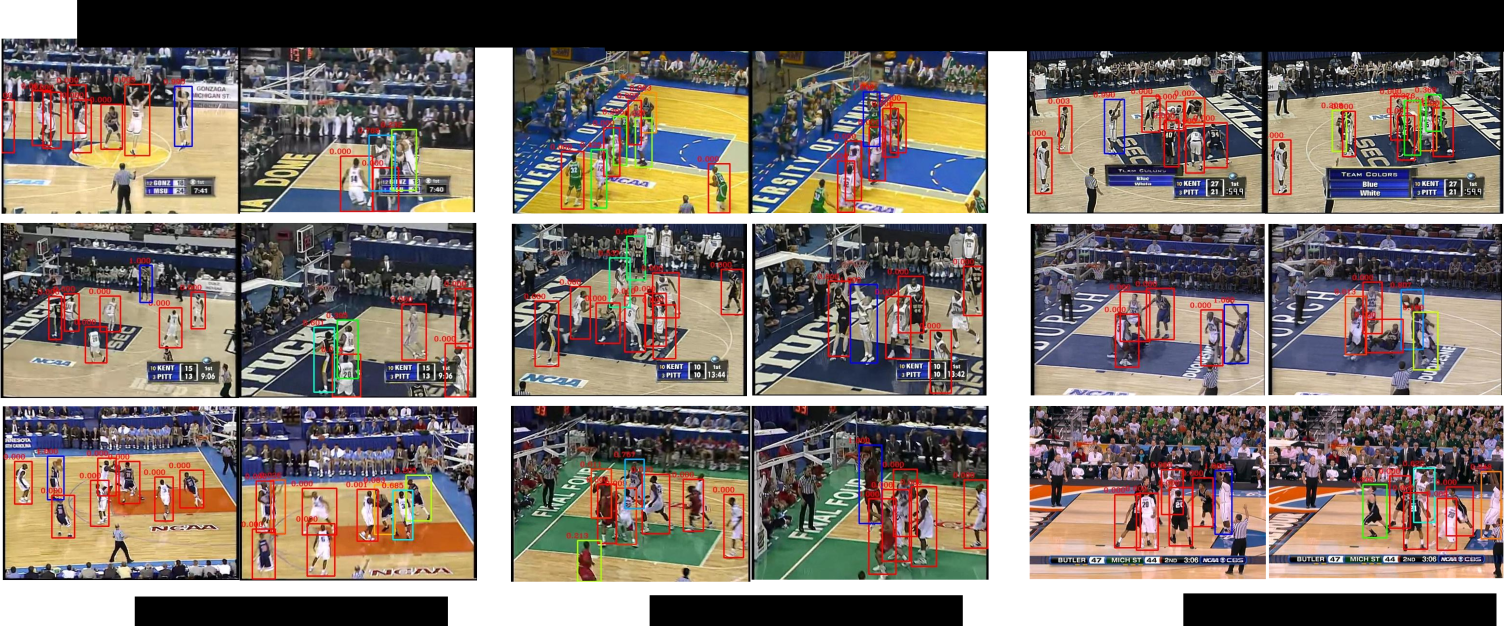
\includegraphics[width=1.0\linewidth]{images/visual_examples.pdf}
\end{center}
   \caption{Visualization of our attention scores at the begining and ending of different events.
Each row of the event corresponds to a different video. It is interesting to note that the model
attends to the shooter when the player makes a shot and to other people under the basket after
the shot is completed.}
\label{fig:visual_attention}
\end{figure*}
% ---------------------------------------------------------------------------------


Apart from good qualitative results,
we are also interested in quantitatively testing this hypothesis.
We collected AMT annotations on $850$ video clips in the test
set, where the annotators were asked to mark the position of the ball
on the frame where the shooter attempts a shot.
This provided us the location of the player shooting the ball.
We used these annotations to evaluate if our ``attention" scores
were capable of classifying the ``shooter" correctly in these frames.
The mean AP for this ``shooter"  classifcation is listed
in Tab.~\ref{tab:attention_res}.

\begin{table}[ht!]
\begin{center}
\small
 \begin{tabular}{|l|c|c|c|}
  \hline
Event            & Rand. ch. & Our no track & Our with track \\ \hline \hline
3-point succ.    & 0.519 & 0.333 & \\ 
3-point fail.    & 0.545 & 0.334 & \\ 
free-throw succ. & 0.772 & 0.376 & \\ 
free-throw fail. & 0.685 & 0.346 & \\  
layup succ.      & 0.627 & 0.386 & \\ 
layup fail.      & 0.605 & 0.382 & \\ 
2-point succ.    & 0.554 & 0.355 & \\ 
2-point fail.    & 0.542 & 0.346 & \\ 
slam dunk succ.  & 0.686 & 0.413 & \\ 
slam dunk fail.  & 0.645 & 0.499 & \\ \hline \hline  
Mean             & 0.377 & 0.618 & \\ \hline
  \end{tabular}
\end{center}
  \caption{Mean average precision for attention evaluation.}
  \label{tab:attention_res}
\end{table}

The scores show that the track-free model is quite consistent in picking
the shooter for several classes like ``free-throw succ./fail",
``layup succ./fail." and ``slam dunk succ.". This is a very
promising result which shows that attention on player detections
alone is capable of localizing the player making the shot. This could be
a useful cue for providing more detailed event descriptions
including the identity and position of the shooter as well.

Since basketball shots are often classified based on the position of the
shooter with respect to the court, we analyze this in
Fig.~\ref{fig:att_heatmap}.  We annotated specific points on the courts and
aligned all the attended boxes for an event to one cannonical image. We have
plotted the resulting heatmap showing the distribution in position of the
attended player with respect to the court. It is interesting to note that
our model consistenly focuses under the basket for a layup, at the free-throw
line for free-throws and outside the 3-point ring for 3-pointers.

% -------- Heat Map for youtube videos
\begin{figure*}[t!]
\begin{center}

   \subfigure[Free-throw success]{
                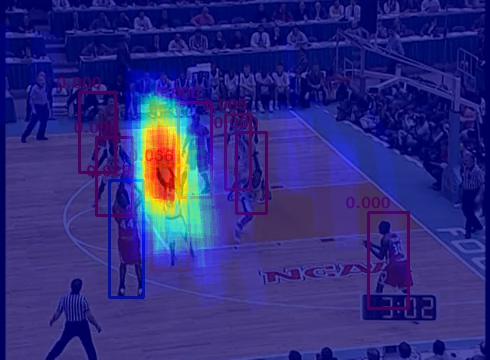
\includegraphics[width=2.2 in]{images/overlayed_freethrow_heatmpa.png}
                \label{fig:heatmap_ft}
    }
   \subfigure[Layup success]{
                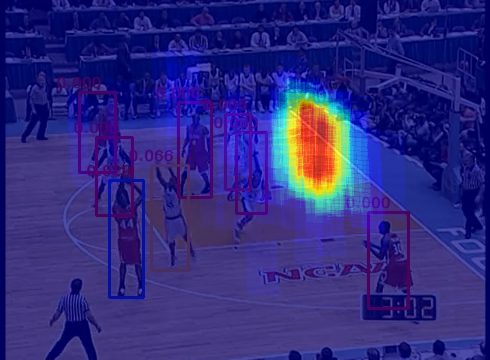
\includegraphics[width=2.2 in]{images/overlayed_layup_heatmpa.png}
                \label{fig:heatmap_lp}
    }
   \subfigure[3-pointer success]{
                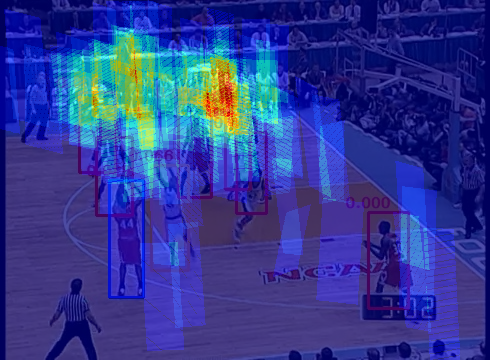
\includegraphics[width=2.2 in]{images/overlayed_3pointer_heatmpa.png}
                \label{fig:heatmap_3p}
    }
\end{center}
   \caption{We show the distribution of the attention over the basketball court
     for different events. We used an affine transform to transform the
     attended player's position to a cannonical frame for visualization.
     Interestingly, the attended court positions are the typical spots from
     which a player would make a shot for the corresponding event.
     \TODO{Also add basketball positions.}
   }
\label{fig:att_heatmap}
\end{figure*}
% ---------------------------------------------------------------------------------


Another interesting observation from Tab.~\ref{tab:attention_res} is that the
attention scores for the tracking based model are less selective in focusing on
the shooter.  We observed that the tracking model is often reluctant to switch
attention between frames and tends to focus on a single player throughout the
event. This biases the model towards players who are present throughout the
event. For instance, in free-throws Fig.~\ref{fig:track_spec_att} we see that
the model always attends to the defender at a specific position, who is visible
throughout the entire event unlike the shooter.

{\small
\bibliographystyle{ieee}
\bibliography{bballbib}
}

\end{document}
